\chapter{Experimente}

Dieses Kapitel beinhaltet die durchgeführten Experimente und die dazugehörigen Resultate. Für die Experimente werden eigens Umgebungen entworfen, um den Agenten mit spezifischen Problemstellungen zu konfrontieren. Dabei handelt es sich um zwei 2D-Umgebungen und eine 3D-Umgebung, in denen der Agent verschiedene Ziele suchen muss. Hierbei soll zum einen die Neural Map im Vergleich zum als Referenz gewählten LSTM betrachtet werden. Darüber hinaus soll ergründet werden, inwiefern die Erweiterung des Schreiboperators die Leistungsfähigkeit der Neural Map verbessert. Den Abschluss des Kapitels bildet eine Untersuchung der Neural Map als reine Speicherstruktur. Dabei wird selbige separiert auf ihre Fähigkeit untersucht, in ihrem internen Speicher eine Karte der Umgebung zu generieren.


\section{2D-Experimente}

Im folgenden Abschnitt wird das Verhalten der Neural Map in zwei eigens dafür konzipierten 2D-Umgebungen untersucht. Die Aufgabe innerhalb dieser Umgebungen besteht im Auffinden von Zielen in verschiedensten Konstellationen. Zunächst werden bis zu vier Ziele in einem hindernisfreien Raum gesucht. Anschließend werden bis zu drei Ziele in einem Labyrinth gesucht. Da in beiden Umgebungen die Ziele in einer bestimmten Reihenfolge aufgefunden werden müssen, kann es passieren, dass der Agent ein erst später zu erreichendes Ziel bereits zu einem früheren Zeitpunkt findet. Auf Basis dieses Ereignisses soll geklärt werden, inwiefern die Neural Map in der Lage ist, solche Ziele zu einem späteren Zeitpunkt möglichst effizient wiederzufinden. Dazu werden verschiedenen Varianten der Neural Map (mit/ohne Erweiterung des Schreiboperators) sowohl untereinander verglichen als auch mit einem LSTM.

Es sei an dieser Stelle noch auf folgenden Sachverhalt hingewiesen, der alle 2D-Experimente dieser Arbeit betrifft. Da der interne Speicher der Neural Map $M$ für alle Experimente in vertikaler und horizontaler Richtung die Größe $15$ aufweist und keine 2D-Umgebung größer als $15 \times 15$ ist, kann auf die in Abschnitt \ref{sec_neural_map} erwähnte Funktion $\psi$ zur Normalisierung der Koordinaten verzichtet werden. Stattdessen entspricht eine Position in der Umgebung exakt derselben Position im internen Speicher. Somit wird für kleinere Umgebungen nur ein entsprechender Teil von $M$ benutzt. Des Weiteren liefert die step-Methode aller Umgebungen nebem dem eigentlichen Zustand $s_t$ auch die aktuelle Position und Orientierung des Agenten. Diese werden jedoch niemals direkt an die Neural Map übergeben, sondern lediglich zum Bereitstellen der Eingabe $M_t^{(x_t,y_t)}$ sowie ggf. $M_t^{(x_{ext_t},y_{ext_t})}$ und für die Update Operation verwendet.

\subsection{Umgebung \glqq One\_Room\_Many\_Goals\_2D\grqq}

\begin{figure}[ht!]
  %\centering
  \begin{subfigure}[c]{0.45\textwidth}
    %\centering
    \includegraphics[keepaspectratio,width=\textwidth]{abbildungen/9x9_ep_start.pdf}
    \subcaption{}
    \label{fig_9x9_ep_start}
  \end{subfigure}
  \begin{subfigure}[c]{0.6\textwidth}
    %\centering
    \includegraphics[keepaspectratio,width=\textwidth]{abbildungen/9x9_sample_obs.pdf}
    \subcaption{}
    \label{fig_9x9_sample_obs}
  \end{subfigure}
  \caption{Die linke Abbildung (a) zeigt einen beispielhaften Episodenbeginn. Das rote Dreieck symbolisiert die Startposition und -orientierung des Agenten, das rote Rechteck die Beobachtung und die farbigen Kreise mit den Nummern die entsprechenden Ziele. Die rechte Abbildung (b) verdeutlicht die binäre Kodierung für die Kanäle 0 und 2 anhand einer beispielhaften Beobachtung.}
\end{figure}


Die Umgebung \glqq One\_Room\_Many\_Goals\_2D\grqq{} ist eine 2D-Umgebung und besteht aus einem Raum, d.h. einer rechteckigen hindernisfreien Fläche, die von einer durchgehenden Wand umgeben ist. In diesem Raum werden zu Beginn jeder Episode wahlweise $2$, $3$ oder $4$ Ziele platziert. Jedes Ziel hat eine eindeutige Nummer zwischen $1$ und $4$. Die Positionen der Ziele werden für jede Episode zufällig neu bestimmt. Dabei gelten folgende Regeln. Zwei aufeinander folgende Ziele dürfen nicht an derselben Position sein, d.h. Ziel 2 darf nicht auf Ziel 1 liegen, Ziel 3 nicht auf Ziel 2 und Ziel 4 nicht auf Ziel 3. Außerdem darf Ziel 1 nicht gleich mit der Startposition des Agenten sein. Der Agent wird zu Beginn jeder Episode auf einer fixen Startposition in der Mitte des Raumes positioniert. Die genauen Koordinaten der Startposition sind von der Größe des Raumes abhängig. Die initiale Blickrichtung des Agenten ist ebenfalls immer gleich, er guckt nach unten. Ein beispielhafter Episodenbeginn für einen Raum der Größe $9 \times 9$ mit 2 Zielen ist in Abbildung \ref{fig_9x9_ep_start} dargestellt. Das rote Dreieck markiert die Startposition und -orientierung des Agenten. Das rote Rechteck umfasst die Felder seiner initialen Beobachtung. Die farbigen Kreise mit den Nummern repräsentieren die beiden Ziele. Die Aufgabe des Agenten besteht dann darin, die Ziele in korrekter Reihenfolge abzulaufen, also zuerst Ziel 1, dann Ziel 2, usw. Hierfür erhält er in Abhängigkeit der Anzahl der Ziele eine entsprechende Belohnung für jedes Ziel. Dabei ist die Belohnung für das letzte Ziel immer signifikant größer als für die Zwischenziele. Auf diese Weise soll der Agent motiviert werden, alle Ziele zu erreichen. Zum Erledigen der Aufgabe steht dem Agenten eine maximale Anzahl an Schritten zur Verfügung. Diese ist abhängig von der Anzahl der Ziele und der Größe der Umgebung und wird stets so gewählt, dass der Agent nicht jedes Feld der Umgebung so oft ablaufen kann, wie es Zile gibt. Das Erreichen des Schrittlimits entspricht dem Übergang in einen Terminalzustand. Für diesen Terminalzustand sowie für jeden anderen getätigten Schritt erhält der Agent einen sogenannten Living-Reward von $-1 / Maximale\_Schrittanzahl$. Durch diesen und durch das Schrittlimit soll der Agent dazu animiert werden, die Aufgabe mit möglichst wenigen Schritten zu absolvieren. In Tabelle \ref{belohnung_ormg} ist der Zusammenhang zwischen der Größe der Umgebung, der Anzahl an Zielen, der Belohnungsstruktur und der maximalen Schrittanzahl übersichtlich zusammengefasst.

\begin{table}[h]
  \begin{tabular}{|>{\centering}m{2cm}|>{\centering}m{1.3cm}|>{\centering}m{1.8cm}|>{\centering}m{1.8cm}|>{\centering}m{1.8cm}|>{\centering}m{1.8cm}|>{\centering}m{2.3cm}|} \hline
    Größe der Umgebung & Anzahl Ziele & Belohnung Ziel 1 & Belohnung Ziel 2 & Belohnung Ziel 3 & Belohnung Ziel 4 & Maximale Schrittanzahl \tabularnewline \hline
    9x9 & 2 & 0.2 & 1.0 & - & - & 75 \tabularnewline \hline
    12x12 & 3 & 0.2 & 0.2 & 1.0 & - & 200 \tabularnewline \hline
    15x15 & 4 & 0.2 & 0.2 & 0.2 & 1.0 & 500 \tabularnewline \hline
  \end{tabular}
  \caption{Übersicht über die verschiedenen Größen der Umgebung \glqq One\_Romm\_Many\_Goals\_2D\grqq{} und die daraus resultierende Anzahl an Zielen, Belohnungsstruktur und maximale Schrittanzahl.}
  \label{belohnung_ormg}
\end{table}

Dem Agenten stehen in jedem Schritt drei mögliche Aktionen zur Verfügung: Gehe einen Schritt bzw. Feld nach vorne, also in Blickrichtung, oder drehe dich um $90\degree$ nach links oder rechts. Dabei kann der Agent nur freie Felder betreten, d.h. wenn der Agent vor sich eine Wand hat und trotzdem einen Schritt nach vorne macht, verändert sich seine Position nicht. Der Zustand $s_t$ ist ein Teilauschnitt der Umgebung in der Größe $(Anzahl\_Ziele + 1) \times 4 \times 3$. Das bedeutet, dass der Agent $4$ Felder geradeaus bzw. in Blickrichtung weit sehen. Zur Seite kann er jeweils 1 Feld sehen, sodass sich mit den Feldern links und rechts des Agenten sowie seinem eigenen die $3$ ergibt. Informationen über die Objekte der Umgebung, d.h. die Wände und die Ziele, sind in Analogie zum Neural Map Paper in den $(Anzahl\_Ziele + 1)$ binärkodierten Kanälen enthalten. Dabei enthält der nullte Kanal Informationen über die Lage der Wände. Hierbei entspricht eine $1$ einem Feld mit einer Wand und eine $0$ einem freien Feld. Die Kanäle $1$ bis $4$ spezifizieren die Positionen der entsprechenden Ziele. Dazu enthält der jeweilige Kanal genau eine $1$ an der Position des Ziels, alle anderen Einträge des Kanals sind $0$. In Abbildung \ref{fig_9x9_sample_obs} wird der Zusammenhang zwischem dem Teilauschnitt der Umgebung und dem daraus resultierenden binärkodierten Zustand $s_t$ für die Kanäle 0 und 2 beispielhaft verdeutlicht.

Folgende Überlegungen spielten beim Design der Umgebung eine Rolle. Zunächst wird durch die zufällige Positionierung der Ziele verhindert, dass es für den Agenten sinvoll ist, immer den gleichen Weg innerhalb der Umgebung zu wählen. Ihm bleibt nichts anderes übrig als, in jeder Episode aufs Neue den Raum zu erkunden. Bei dieser Erkundung kann es dann passieren, dass er Ziele sieht, die er erst zu einem späteren Zeitpunkt erreichen muss. Diese Situationen sind für die folgenden Untersuchungen von besonderem Interesse. Es wäre wünschenswert, wenn der Agent die Information über ein später zu erreichendes Ziel in seinem internen Speicher ablegen könnte und zu dem Zeitpunkt, wenn das entsprechende Ziel an der Reihe ist, wieder abrufen könnte. Basierend darauf sollte er im Idealfall dann einen möglichst direkten Weg zu dem entsprechenden Ziel wählen. Um die Wahrscheinlichkeit für solche Situationen zu erhöhen wird in den folgenden Experimenten sowohl die Anzahl der Ziele sukzessive erhöht, als auch die Größe der Umgebung. Durch die Vergrößerung der Umgebung benötigt der Agent mehr Schritte zur Erkundung selbiger, wobei mit jedem Schritt die Möglichkeit besteht, ein später zu erreichendes Ziel zu beobachten. Die Wahrscheinlichkeit dafür wird durch eine höhere Anzahl an Zielen noch zusätzlich erhöht. Außerdem kann auf diese Weise auch noch untersucht werden, wie gut der Agent mehrere zukünftige Ziele in der Neural Map abspeichern kann.

In den folgenden Experimenten werden vier verschiedene Varianten der Neural Map mit einem LSTM als Referenz verglichen. Die erste Variante der Neural Map entspricht der in Abschnitt \ref{sec_nm_impl} beschriebenen Implementierung. Durch die in Abschnitt \ref{sec_write_ext} eingeführte Erweitertung des Schreiboperators entsteht die zweite Variante. Die beiden weiteren Varianten entstehen dadurch, dass für den Schreiboperator und seine Erweiterung die in Abschnitt \ref{sec_neural_map} präsentierte GRU-based Local Write Operation verwendet wird. Die zum Training verwendeten Hyperparameter des PPO Algorithmus können der Tabelle \ref{hyperparam_ppo_ormg} entnommen werden. Diese sind für alle Experimente basierend auf der Umgebung \glqq One\_Room\_Many\_Goals\_2D\grqq{} und für alle zu untersuchenden Modelle gleich. Lediglich der Parameter $total\_timesteps$, der die für das Training zur Verfügung stehende Gesamtanzahl an Schritten spezifiziert, ist in Abhängigkeit der Umgebungsgröße und Anzahl an Zielen gewählt worden. Somit wird dieser auch in den entsprechenden Unterabschnitten angegeben. Im Anschluss an das Training wird das Modell für $10^5$ Zeitschritte in der jeweiligen Umgebung ausgeführt. Da angenommen wird, dass im internen Speicher der Neural Map $M_t$ eine Karte der Umgebung generiert wird, wird er beim Erreichen eines Terminalzustandes in seinen Initialzustand zurückgesetzt. In diesem enthält der Speicher in allen Einträgen Nullen. Dieses Zurücksetzen des Speichers wird sowohl im Training als auch in der Evaluation durchgeführt.

\begin{table}[h]
  \begin{center}
    \begin{tabular}{1 1}
      \hline
      nsteps & $512$ \\
      ent\_coef & $0.025$ \\
      lr & $0$ \\
      vf\_coef & $0$ \\
      max\_grad\_norm & $0$ \\
      gamma & $0.99$ \\
      noptepochs & $1$ \\
      cliprange & $0.0$ \\
      \hline
    \end{tabular}
  \end{center}
  \caption{Übersicht über die zum Training der Umgebung \glqq One\_Room\_Many\_Goals\_2D\grqq{} verwendeten Hyperparameter des PPO Algorithmus.}
  \label{hyperparam_ppo_ormg}
\end{table}


\subsubsection{Umgebungsgröße 9x9 und 2 Ziele}
Für das erste Experiment werden in einer Umgebung der Größe $9 \times 9$ zwei Ziele platziert. Die Abbildungen \ref{fig_9x9_ep_start} und \ref{fig_9x9_sample_obs} zeigen beispielhaft den Episodenbeginn und einen zufälligen Zeitschritt für die entsprechende Umgebungsgröße und Zielanzahl. Alle Modelle werden zunächst für $2,5\cdot10^6$ Zeitschritte trainiert und anschließend für $10^6$ ausgeführt zu Evaluationszwecken. Um die Leistungsfähigkeit der verschiedenen Modelle zu vergleichen, werden während der Evaluation sowohl die pro Episode erhaltenen Rewards als auch die Länge der Episoden aufgezeichnet. Durch die zufällige Platzierung der Ziele variiert auch die Anzahl benötigter Schritte pro Episode und infolgedessen auch der Reward pro Episode. Deshalb wird von diesen beiden Werten jeweils der Durchschnitt über alle erfolgreichen Episoden betrachtet. In Tabelle \ref{results9x9} sind die entsprechenden Ergebnisse aller Modelle zusammengefasst. Darüber hinaus enthält sie auch noch die Anzahl erfolgreich absolvierter Episoden. Hierbei fällt als Erstes auf, dass die Neural Map mit der Erweiterung des Schreiboperators (Neural Map + extW) die besten Ergebnisse erzielt. Sie absolviert in den $10^6$ zur Verfügung stehenden Zeitschritten 4338 erfolgreiche Episoden und benötigt im Durchschnitt für eine erfolgreich absolvierte Episode 21,73 Schritte. Dabei erreicht sie einen durchscnittlichen Reward von 0,91. Im Vergleich zur zweitbesten Variante (Neural Map + extW + GRU) benötigt sie somit ungefähr 2 Schritte weniger pro Episode. Die Grundvariante der Neural Map tätigt sogar ungefähr 3 Schritte mehr und die Referenz, das LSTM, ungefähr 5 Schritte. Die Verwendung der GRU-basierten Local Write Operation bringt hingegen keine Verbesserung und zwar sowohl bezüglich der Grundvariante der Neural Map als auch der Variante mit dem erweiterten Schreiboperator. Abschließend kann noch festgehalten werden, dass alle untersuchten Varianten der Neural Map bessere Ergebnisse erzielen als das LSTM.

\begin{table}[ht!]
  \begin{tabular}{|>{\centering}m{5cm}|>{\centering}m{2.2cm}|>{\centering}m{3.5cm}|>{\centering}m{3.5cm}|} \hline
    Modell  & Anzahl erfolgreicher Episoden & Durchschnittliche Schrittanzahl pro erfolgreicher Episode & Durchschnittlicher Reward pro erfolgreicher Episode \tabularnewline \hline
    LSTM & 3540 & 26,40 & 0,85 \tabularnewline \hline
    Neural Map & 3854 & 24,80 & 0,87 \tabularnewline \hline
    Neural Map + extW & \textbf{4338} & \textbf{21,73} & \textbf{0,91} \tabularnewline \hline
    Neural Map + GRU & 3717 & 25,12 & 0,86 \tabularnewline \hline
    Neural Map + extW + GRU & 4067 & 23,67 & 0,88 \tabularnewline \hline
  \end{tabular}
  \caption{Übersicht über die Anzahl erfolgreicher Episoden, deren durchschnittliche Länge und Reward für die Umgebung \glqq One\_Romm\_Many\_Goals\_2D\grqq{} in der Größe $9 \times 9$ mit 2 Zielen.}
  \label{results9x9}
\end{table}

Um einen detailiertern Einblick in das Verhalten der verschiedenen Modelle zu gewinnen, werden während der Evaluation nicht nur der Reward und die Schrittanzahl pro Episode aufgezeichnet, sondern auch die Observationen bzw. Zustände $s_t$, die Rewards $R_t$ und die Positionen des Agenten $(x_t,y_t)$. Hieraus lässt sich für jede Episode der gelaufene Weg des Agenten nachvollziehen. Darüber hinaus können mit diesen Daten die Positionen der Ziele rekonstruiert werden.

Da der Fokus des Experiments darauf liegt, inwiefern der Agent seinen internen Speicher zur Wegfindung nutzen kann, wird im folgenden der Weg vom ersten zum zweiten Ziel detailierter betrachtet. Dies geschieht aus den folgenden Gründen. Zu Beginn jeder Episode verfügt der Agent logischerweise über keinerlei Wissen bezüglich der Positionen der Ziele. Somit muss er den Raum jedes mal aufs Neue erkunden. Dabei wird er dann irgendwann zufällig auf sein erstes Ziel stoßen. Die dafür benötigte Anzahl von Schritten hängt jedoch in erster Linie von der zufälligen Position des Zieles ab und nicht vom Inhalt bzw. der Nutzung des internen Speichers. Dabei wird angenommen, dass der Agent die Umgebung möglichst effizient erkundet, d.h. gewisse Felder bzw. Bereiche werden nicht mehrfach betreten. Auch wenn der interne Speicher bei einer effizienten Erkundung durchaus von Nutzen sein kann, wird dies wird jedoch vernachlässigt. Somit ist der eigentliche Weg zum ersten Ziel von nachgeordnetem Interesse. Allerdings besteht die Möglichkeit, dass der Agent, während er auf der Suche nach dem ersten Ziel ist, das Zweite bereits sieht. Ist dies der Fall, so ist im Optimalfall der Weg vom ersten zum zweiten Ziel kein rein zufälliger Erkundungsweg mehr, sondern ein zielgerichtetes Wiederauffinden eines zuvor bereits beobachteten Ziels. Um den Weg des Agenten vom ersten zum zweiten Ziel zu bewerten, wird zunächst für jede Episode die optimale Anzahl an Aktionen ermittelt, die für diesen Weg benötigt wird. Diese ergibt sich in erster Linie aus dem Abstand der beiden Ziele, d.h. aus den Beträgen der Differenzen der x- und y-Koordinaten, und den dafür benötigten Schritten. Darüber hinaus werdem eventuell noch Drehungen benötigt. In Abhängigkeit der Orientierung des Agenten und der Lage der Ziele ergibt sich die Anzahl benötigter Drehungen entweder zu Null, Eins oder Zwei. Um auf aufwendige Fallunterscheidungen verzichten zu können, wird einfach immer von zwei Drehungen ausgegangen. Somit kann eine pessimistische Schätzung der optimalen Anzahl an Aktionen um von Ziel i zu Ziel j zu kommen mit der folgenden Formel berechnet werden:

\begin{equation}
  Optimale\_Schrittanzahl_{i,j} = |x_i - x_j| + |y_i - y_j| + 2
  \label{opt_steps_i_to_j}
\end{equation}

Von diesem Wert wird anschließend der Durchschnitt über alle Episoden gebildet. Ebenso wird für jede Episode die tatsächliche Anzahl benötigter Schritte für den entsprechenden Weg bestimmt, sowie der Durchschnitt über alle Episoden. Diese beiden Durchschnittswerte sowie deren Differenz, die der Anzahl zusätzlicher Schritte entspricht, sind für die betrachteten Modelle in Tabelle \ref{results9x9_1_to_2} zusammengefasst. Es zeigt sich, dass die durchschnittliche optimale Schrittanzahl für alle Modelle sehr ähnlich ist. Die Spannweite ist kleiner als 0,1 Schritte. Somit ist die durchschnittliche Entfernung zwischen den beiden Zielen in den betrachteten Episoden bei allen Modellen sehr ähnlich. Dies verleiht den Werten der tatsächlichen Schrittanzahl bzw. der Anzahl zusätzlicher Schritte mehr Aussagekraft, da diese wiederum immer in Bezug zur optimalen Schrittanzahl betrachtet werden müssen. So macht es einen erheblichen Unterschied, ob der Agent beispielsweise im Durchschnitt 5 zusätzliche Schritte tätigt bezogen auf einen optimalen Weg von 5 oder von 50 Schritten. Die Ergebnisse spiegeln die Gesamtlesitungen der verschiedenen Modelle aus Tabelle \ref{results9x9} wieder. Die Neural Map mit der Erweiterung des Schreiboperators benötigt im Durchschnitt die wenigsten zusätzlichen Schritte für den Weg von Ziel 1 zu Ziel 2. Darüber hinaus kommen alle Varianten der Neural Map mit weniger zusätzlichen Schritten aus als das LSTM.

\begin{table}[ht!]
  \begin{tabular}{|>{\centering}m{5cm}|>{\centering}m{2.9cm}|>{\centering}m{2.9cm}|>{\centering}m{3.3cm}|} \hline
    Modell  & Durchschnittliche optimale Schrittanzahl & Durchschnittliche tatsächliche Schrittanzahl & Durchschnittliche Anzahl zusätzlicher Schritte \tabularnewline \hline
    LSTM & 6,66 & 13,66 & 7,00 \tabularnewline \hline
    Neural Map & 6,75 & 13,11 & 6,36 \tabularnewline \hline
    Neural Map + extW & 6,71 & \textbf{12,40} & \textbf{5,69} \tabularnewline \hline
    Neural Map + GRU & 6,68 & 13,26 & 6,58 \tabularnewline \hline
    Neural Map + extW + GRU & 6,72 & 12,87 & 6,15 \tabularnewline \hline
  \end{tabular}
  \caption{Übersicht über die optimale Schrittanzahl, die tatsächliche Schrittanzahl und die Anzahl zusätzlicher Schritte bezogen auf den Weg von Ziel 1 zu Ziel 2 in der Umgebung \glqq One\_Romm\_Many\_Goals\_2D\grqq{} in der Größe $9 \times 9$ mit 2 Zielen.}
  \label{results9x9_1_to_2}
\end{table}

Anstatt den Durchschnitt über alle Episoden für den Weg vom ersten zum zweiten Ziel zu betrachten, werden die Episoden im folgenden in drei Mengen aufgeteilt. Alle Episoden, in denen bei der Suche nach dem ersten Ziel das zweite Ziel zu keinem Zeitpunkt gesichtet wurde, bilden die erste Menge. Diese Menge kann in gewisser Weise als Referenz für die beiden anderen Mengen betrachtet werden, da sich bei ihr die zufällige Suche für das zweite Ziel fortsetzt. Die zweite Menge enthält alle Episoden, in denen der Agent mindestens einmal über das zweite Ziel drüber gelaufen ist, d.h. das sich der Agent zu mindestens einem Zeitpunkt an exakt derselben Position wie Ziel 2 befunden hat. Hat der Agent das zweite Ziel lediglich gesichtet, ist jedoch nicht drüber gelaufen, so ist die entsprechende Episode Teil der dritten Menge. Für die drei Mengen werden die Bezeichnungen \glqq Ziel 2 nie beobachtet\grqq{}, \glqq Ziel 2 besucht\grqq{} und \glqq Ziel 2 gesehen\grqq{}. Für die Zuordnung der Episoden zu den jeweiligen Mengen werden alle zu einer Episode gehörenden Observationen betrachtet und hiervon wiederum speziell die mit dem zweiten Kanal bzw. Ziel korrespondierenden. Die Unterscheidung zwischen \glqq Ziel\grqq{} besucht und \glqq Ziel\grqq{} gesehen wird vorgenommen, da die Grundvariante der Neural Map nur die Speicherposition beschreibt, die der aktuellen Position des Agenten entspricht. Allerdings enthält die Observation des Agenten nicht nur Informationen über das Feld, auf dem er sich aktuell befindet, sondern auch noch über weitere Felder der Umgebung. Somit soll durch diese Unterscheidung untersucht werden, ob Informationen der Umgebung, die der aktuellen Position des Agenten entsprechen, anders verarbeitet werden beim Beschreiben des internen Speichers als die restlichen Informationen der Observation. Dazu wird für jede Episode wieder mit der Formel \ref{opt_steps_i_to_j} die optimale Schrittanzahl berechnet. Ebenso wird für jede Episode wieder die tatsächliche Schrittanzahl und die Anzahl zusätzlicher Schritte bestimmt. In Tabelle \ref{results9x9_1_to_2_per_M} sind die Durchschnittswerte der optimalen (Opt) und zusätzlichen Schrittanzahl (Differenz) für die verschiedenen Mengen für alle Modelle dargestellt. Dabei ist die Differenz zwischen optimaler und tatsächlicher Schrittanzahl einmal absolut (abs.) und einmal relativ (rel.) angegeben. Für die relative Differenz fungiert die optimale Schrittanzahl als Bezugsgröße, d.h. der absolute Wert durch diese dividiert und anschließend mit Hundert multipliziert für eine Angabe in Prozent. Bei den Ergebnissen fällt als Erstes auf, dass die optimale Schrittanzahl zwischen den Zielen für die jeweilige Menge relativ ähnlich ist. So liegt sie für die Menge \glqq Ziel 2 nie beobachtet\grqq{} zwischen 7,52 und 7,62, für die Menge \glqq Ziel 2 besucht\grqq{} zwischen 6,62 und 6,82 und für die Menge \glqq Ziel 2 gesehen\grqq{} zwischen 4,0 und 4,73. Darüber hinaus ist es auffällig, dass in den Episoden der Menge \glqq Ziel 2 gesehen\grqq{} die Ziele 1 und 2 wesentlich näher beieinander liegen als in den anderen beiden Mengen und alle Modelle in dieser Menge die geringste Anzahl zusätzlicher Schritte benötigen. Bezüglich der beiden Mengen \glqq Ziel 2 nie beobachtet\grqq{} und \glqq Ziel 2 besucht\grqq{} lässt sich bei den verschiedenen Modellen keine Systematik hinsichtlich der Anzahl zusätzlicher Schritte feststellen. Manche Modelle benötigen in der einen Menge weniger zusätzliche Schritte, manchen in der Anderen.

\begin{table}
  \begin{tabular}{|c|c|c|c|c|c|c|c|c|c|}
    \hline
    \multirow{3}{*}{Modell} & \multicolumn{3}{|c|}{Ziel 2 nie beobachtet} & \multicolumn{3}{|c|}{Ziel 2 besucht} & \multicolumn{3}{|c|}{Ziel 2 gesehen} \\ \cline{2-10}
    & \multirow{2}{*}{Opt} & \multicolumn{2}{|c|}{Differenz} & \multirow{2}{*}{Opt} & \multicolumn{2}{|c|}{Differenz} & \multirow{2}{*}{Opt} & \multicolumn{2}{|c|}{Differenz} \\ \cline{3-4} \cline{6-7} \cline{9-10}
    & & abs. & rel. & & abs. & rel. & & abs. & rel. \\ \hline
    LSTM & 7,52 & 9,61 & 128\% & 6,67 & 6,26 & 94\% & 4,42 & 3,03 & 69\% \\ \hline
    Neural Map & 7,53 & 6,65 & 88\% & 6,82 & 7,32 & 107\% & 4,00 & 1,44 & 36\% \\ \hline
    Neural Map + extW & 7,62 & 6,91 & 91\% & 6,78 & 5,69 & 84\% & 4,73 & 2,68 & 56\% \\ \hline
    Neural Map + GRU & 7,58 & 7,61 & 100\% & 6,65 & 7,01 & 105\% & 4,11 & 1,65 & 40\% \\ \hline
    Neural Map + extW + GRU & 7,60 & 7,16 & 94\% & 6,62 & 6,35 & 96\% & 4,64 & 2,75 & 59\% \\ \hline
  \end{tabular}
  \caption{Übersicht über die optimale (Opt) und zusätzliche Schrittanzahl (Differenz) für den Weg von Ziel 1 zu Ziel 2 aufgeteilt in die drei Mengen \glqq Ziel 2 nie beobachtet\grqq{}, \glqq Ziel 2 besucht\grqq{} und \glqq Ziel 2 gesehen\grqq{} für die Umgebung \glqq One\_Romm\_Many\_Goals\_2D\grqq{} in der Größe $9 \times 9$ mit 2 Zielen.}
  \label{results9x9_1_to_2_per_M}
\end{table}


\subsubsection{Umgebungsgröße 12x12 und 3 Ziele}

\begin{figure}[ht!]
  \centering
  \includegraphics[keepaspectratio,width=0.6\textwidth]{abbildungen/12x12_ep_start.pdf}
  %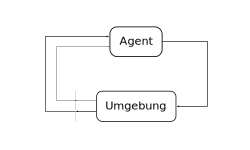
\includegraphics[height=0.5\textwidth, width=0.9\textwidth]{abbildungen/schnittstelle_agent_umgebung.pdf}
  \caption{Die Abbildung zeigt einen beispielhaften Episodenbeginn für die Umgebungsgröße $12 \times 12$ und 3 Ziele. Das rote Dreieck symbolisiert Startposition und -orientierung des Agenten, das rote Rechteck seine initiale Beobachtung und die farbigen Kreise mit den Nummern die entsprechenden Ziele. Die gestreichelten Pfeile zeigen einen möglichen optimalen Weg.}
  \label{fig_12x12_ep_start}
\end{figure}

Als nächstes wird die Größe der Umgebung auf $12 \times 12$ erhöht und es werden 3 Ziele in ihr platziert. Dadurch wird die Aufgabe für den Agenten anspruchsvoller. Ein beispielhafter Episodenbeginn ist in Abbildung \ref{fig_12x12_ep_start} dargestellt. Neben der Startposition des Agenten, seiner initialen Beobachtung und der Lage der Ziele ist ein möglicher optimaler Weg des Agenten durch die gestrichelten roten Pfeile angedeutet. Das beschreiten dieses Wegs ist jedoch höchst unwahrscheinlich, da der Agent hierfür die Lage der Ziele bereits kennen müsste. Dies ist jedoch selbstverständlich nicht der Fall. Der optimale Weg ist nur zur Veranschaulichung der Problemkomplexität eingezeichnet. In dieser Konfiguration werden alle Modelle für $5\cdot10^6$ Zeitschritte trainiert und anschließend wieder für $10^6$ Zeitschritte evaluiert. Die Auswertung entspricht im Wesentlichen der des vorangegangenen Abschnitts. Zunächst wird die Gesamtleistung der verschiedenen Modelle anhand der Anzahl erfolgreich absolvierter Episoden, der durchschnittlichen Länge und des durchschnittlichen Rewards pro erfolgreicher Episode beurteilt. Die entsprechenden Ergebnisse können der Tabelle \ref{results12x12} entnommen werden. Die beiden Varianten mit der Erweiterung des Schreiboperators erzielen bessere Ergebnisse als die beiden Variante ohne. Dabei erreicht die Variante der Neural Map mit der Erweiterung des Schreiboperators unter Verwendung des GRU-basierten Schreiboperators das beste Resultat mit durchschnittlich 84,08 Schritten pro erfolgreicher Episode. Insgesamt verbessert in dieser Konfiguration der Umgebung die Benutzung der GRU-basierten Schreiboperation die jeweilige Neural Map Variante. Des Weiteren liefern alle Varianten der Neural Map wieder bessere Ergebnis als das LSTM.

\begin{table}[ht!]
  \begin{tabular}{|>{\centering}m{5cm}|>{\centering}m{2.2cm}|>{\centering}m{3.5cm}|>{\centering}m{3.5cm}|} \hline
    Modell  & Anzahl erfolgreicher Episoden & Durchschnittliche Schrittanzahl pro erfolgreicher Episode & Durchschnittlicher Reward pro erfolgreicher Episode \tabularnewline \hline
    LSTM & 923 & 92,36 & 0,94 \tabularnewline \hline
    Neural Map & 975 & 88,53 & 0,96 \tabularnewline \hline
    Neural Map + extW & 995 & 86,73 & 0,97 \tabularnewline \hline
    Neural Map + GRU & 983 & 88,11 & 0,96 \tabularnewline \hline
    Neural Map + extW + GRU & \textbf{1053} & \textbf{84,08} & \textbf{0,98} \tabularnewline \hline
  \end{tabular}
  \caption{Übersicht über die Anzahl erfolgreicher Episoden, deren durchschnittliche Länge und Reward für die Umgebung \glqq One\_Romm\_Many\_Goals\_2D\grqq{} in der Größe $12 \times 12$ mit 3 Zielen.}
  \label{results12x12}
\end{table}

Mit der gleichen Begründung wie im vorherigen Abschnitt wird als nächstes wieder der Weg vom ersten zum zweiten Ziel detailierter untersucht. Dabei werden die Episoden wieder in die drei Mengen \glqq Ziel 2 nie beobachtet\grqq{}, \glqq Ziel 2 besucht\grqq{} und \glqq Ziel 2 gesehen\grqq{} aufgeteilt und es wird für jede Menge die durchschnittliche optimale Schrittanzahl und die durchschnittliche Anzahl zusätzlicher Schritte berechnet. Die entsprechenden Ergebnisse sind in Tabelle \ref{results12x12_1_to_2_per_M} dargestellt.

\begin{table}
  \begin{tabular}{|c|c|c|c|c|c|c|c|c|c|}
    \hline
    \multirow{3}{*}{Modell} & \multicolumn{3}{|c|}{Ziel 2 nie beobachtet} & \multicolumn{3}{|c|}{Ziel 2 besucht} & \multicolumn{3}{|c|}{Ziel 2 gesehen} \\ \cline{2-10}
    & \multirow{2}{*}{Opt} & \multicolumn{2}{|c|}{Differenz} & \multirow{2}{*}{Opt} & \multicolumn{2}{|c|}{Differenz} & \multirow{2}{*}{Opt} & \multicolumn{2}{|c|}{Differenz} \\ \cline{3-4} \cline{6-7} \cline{9-10}
    & & abs. & rel. & & abs. & rel. & & abs. & rel. \\ \hline
    LSTM & 9,17 & 23,31 & 254\% & 8,57 & 23,09 & 270\% & 4,40 & 11,62 & 264\% \\ \hline
    Neural Map & 8,35 & 26,07 & 312\% & 7,83 & 21,85 & 279\% & 4,08 & 5,63 & 138\% \\ \hline
    Neural Map + extW & 9,07 & 22,92 & 253\% & 8,19 & 22,73 & 277\% & 3,93 & 5,56 & 141\% \\ \hline
    Neural Map + GRU & 8,71 & 24,28 & 279\% & 8,28 & 22,21 & 268\% & 3,66 & 7,41 & 202\% \\ \hline
    Neural Map + extW + GRU & 9,13 & 23,87 & 261\% & 8,38 & 21,39 & 257\% & 4,5 & 9,34 & 208\% \\ \hline
  \end{tabular}
  \caption{Übersicht über die optimale (Opt) und zusätzliche Schrittanzahl (Differenz) für den Weg von Ziel 1 zu Ziel 2 aufgeteilt in die drei Mengen \glqq Ziel 2 nie beobachtet\grqq{}, \glqq Ziel 2 besucht\grqq{} und \glqq Ziel 2 gesehen\grqq{} für die Umgebung \glqq One\_Romm\_Many\_Goals\_2D\grqq{} in der Größe $12 \times 12$ mit 3 Zielen.}
  \label{results12x12_1_to_2_per_M}
\end{table}



\begin{table}
  \begin{tabular}{|c|c|c|c|c|c|c|c|c|c|}
    \hline
    \multirow{3}{*}{Modell} & \multicolumn{3}{|c|}{Ziel 2 nie beobachtet} & \multicolumn{3}{|c|}{Ziel 2 besucht} & \multicolumn{3}{|c|}{Ziel 2 gesehen} \\ \cline{2-10}
    & \multirow{2}{*}{Opt} & \multicolumn{2}{|c|}{Differenz} & \multirow{2}{*}{Opt} & \multicolumn{2}{|c|}{Differenz} & \multirow{2}{*}{Opt} & \multicolumn{2}{|c|}{Differenz} \\ \cline{3-4} \cline{6-7} \cline{9-10}
    & & abs. & rel. & & abs. & rel. & & abs. & rel. \\ \hline
    LSTM & 9,74 & 26,93 & 276\% & 8,69 & 21,64 & 249\% & 5,18 & 14,36 & 277\% \\ \hline
    Neural Map & 9,98 & 25,06 & 251\% & 8,21 & 21,68 & 264\% & 4,70 & 14,78 & 314\% \\ \hline
    Neural Map + extW & 9,59 & 24,29 & 253\% & 8,37 & 20,47 & 244\% & 5,51 & 14,12 & 256\% \\ \hline
    Neural Map + GRU & 9,83 & 29,57 & 301\% & 8,62 & 20,36 & 236\% & 5,85 & 8,68 & 148\% \\ \hline
    Neural Map + extW + GRU & 9,85 & 25,47 & 258\% & 8,34 & 17,22 & 207\% & 4,41 & 5,72 & 130\% \\ \hline
  \end{tabular}
  \caption{Übersicht über die optimale (Opt) und zusätzliche Schrittanzahl (Differenz) für den Weg von Ziel 2 zu Ziel 3 aufgeteilt in die drei Mengen \glqq Ziel 2 nie beobachtet\grqq{}, \glqq Ziel 2 besucht\grqq{} und \glqq Ziel 2 gesehen\grqq{} für die Umgebung \glqq One\_Romm\_Many\_Goals\_2D\grqq{} in der Größe $12 \times 12$ mit 3 Zielen.}
  \label{results12x12_2_to_3_per_M}
\end{table}



\subsubsection{Umgebungsgröße 15x15 und 4 Ziele}


\begin{figure}[ht!]
  \centering
  \includegraphics[keepaspectratio,width=0.6\textwidth]{abbildungen/15x15_ep_start.pdf}
  %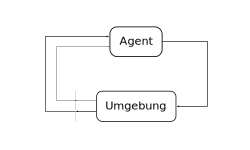
\includegraphics[height=0.5\textwidth, width=0.9\textwidth]{abbildungen/schnittstelle_agent_umgebung.pdf}
  \caption{Die Abbildung zeigt einen beispielhaften Episodenbeginn für die Umgebungsgröße $15 \times 15$ und 4 Ziele. Das rote Dreieck symbolisiert Startposition und -orientierung des Agenten, das rote Rechteck seine initiale Beobachtung und die farbigen Kreise mit den Nummern die entsprechenden Ziele. Die gestreichelten Pfeile zeigen einen möglichen optimalen Weg.}
  \label{fig_12x12_ep_start}
\end{figure}
total\_timesteps: $10\cdot10^6$

\begin{table}[ht!]
  \begin{tabular}{|>{\centering}m{5cm}|>{\centering}m{2.2cm}|>{\centering}m{3.5cm}|>{\centering}m{3.5cm}|} \hline
    Modell  & Anzahl erfolgreicher Episoden & Durchschnittliche Schrittanzahl pro erfolgreicher Episode & Durchschnittlicher Reward pro erfolgreicher Episode \tabularnewline \hline
    LSTM & 329 & 269,75 & 1,08 \tabularnewline \hline
    Neural Map & 365 & 242,12 & 1,12 \tabularnewline \hline
    Neural Map + extW & 397 & 230,25 & 1,14 \tabularnewline \hline
    Neural Map + GRU & 360 & 239,43 & 1,12 \tabularnewline \hline
    Neural Map + extW + GRU & \textbf{404} & \textbf{224,65} & \textbf{1,15} \tabularnewline \hline
  \end{tabular}
  \caption{Übersicht über die Anzahl erfolgreicher Episoden, deren durchschnittliche Länge und Reward für die Umgebung \glqq One\_Romm\_Many\_Goals\_2D\grqq{} in der Größe $15 \times 15$ mit 4 Zielen.}
  \label{results15x15}
\end{table}

\begin{table}
  \begin{tabular}{|c|c|c|c|c|c|c|c|c|c|}
    \hline
    \multirow{3}{*}{Modell} & \multicolumn{3}{|c|}{Ziel 2 nie beobachtet} & \multicolumn{3}{|c|}{Ziel 2 besucht} & \multicolumn{3}{|c|}{Ziel 2 gesehen} \\ \cline{2-10}
    & \multirow{2}{*}{Opt} & \multicolumn{2}{|c|}{Differenz} & \multirow{2}{*}{Opt} & \multicolumn{2}{|c|}{Differenz} & \multirow{2}{*}{Opt} & \multicolumn{2}{|c|}{Differenz} \\ \cline{3-4} \cline{6-7} \cline{9-10}
    & & abs. & rel. & & abs. & rel. & & abs. & rel. \\ \hline
    LSTM & 9,74 & 26,93 & 276\% & 8,69 & 21,64 & 249\% & 5,18 & 14,36 & 277\% \\ \hline
    Neural Map & 9,98 & 25,06 & 251\% & 8,21 & 21,68 & 264\% & 4,70 & 14,78 & 314\% \\ \hline
    Neural Map + extW & 9,59 & 24,29 & 253\% & 8,37 & 20,47 & 244\% & 5,51 & 14,12 & 256\% \\ \hline
    Neural Map + GRU & 9,83 & 29,57 & 301\% & 8,62 & 20,36 & 236\% & 5,85 & 8,68 & 148\% \\ \hline
    Neural Map + extW + GRU & 9,85 & 25,47 & 258\% & 8,34 & 17,22 & 207\% & 4,41 & 5,72 & 130\% \\ \hline
  \end{tabular}
  \caption{Übersicht über die optimale (Opt) und zusätzliche Schrittanzahl (Differenz) für den Weg von Ziel 1 zu Ziel 2 aufgeteilt in die drei Mengen \glqq Ziel 2 nie beobachtet\grqq{}, \glqq Ziel 2 besucht\grqq{} und \glqq Ziel 2 gesehen\grqq{} für die Umgebung \glqq One\_Romm\_Many\_Goals\_2D\grqq{} in der Größe $15 \times 15$ mit 4 Zielen.}
  \label{results15x15_2_to_3_per_M}
\end{table}

\begin{table}
  \begin{tabular}{|c|c|c|c|c|c|c|c|c|c|}
    \hline
    \multirow{3}{*}{Modell} & \multicolumn{3}{|c|}{Ziel 2 nie beobachtet} & \multicolumn{3}{|c|}{Ziel 2 besucht} & \multicolumn{3}{|c|}{Ziel 2 gesehen} \\ \cline{2-10}
    & \multirow{2}{*}{Opt} & \multicolumn{2}{|c|}{Differenz} & \multirow{2}{*}{Opt} & \multicolumn{2}{|c|}{Differenz} & \multirow{2}{*}{Opt} & \multicolumn{2}{|c|}{Differenz} \\ \cline{3-4} \cline{6-7} \cline{9-10}
    & & abs. & rel. & & abs. & rel. & & abs. & rel. \\ \hline
    LSTM & 9,74 & 26,93 & 276\% & 8,69 & 21,64 & 249\% & 5,18 & 14,36 & 277\% \\ \hline
    Neural Map & 9,98 & 25,06 & 251\% & 8,21 & 21,68 & 264\% & 4,70 & 14,78 & 314\% \\ \hline
    Neural Map + extW & 9,59 & 24,29 & 253\% & 8,37 & 20,47 & 244\% & 5,51 & 14,12 & 256\% \\ \hline
    Neural Map + GRU & 9,83 & 29,57 & 301\% & 8,62 & 20,36 & 236\% & 5,85 & 8,68 & 148\% \\ \hline
    Neural Map + extW + GRU & 9,85 & 25,47 & 258\% & 8,34 & 17,22 & 207\% & 4,41 & 5,72 & 130\% \\ \hline
  \end{tabular}
  \caption{Übersicht über die optimale (Opt) und zusätzliche Schrittanzahl (Differenz) für den Weg von Ziel 2 zu Ziel 3 aufgeteilt in die drei Mengen \glqq Ziel 2 nie beobachtet\grqq{}, \glqq Ziel 2 besucht\grqq{} und \glqq Ziel 2 gesehen\grqq{} für die Umgebung \glqq One\_Romm\_Many\_Goals\_2D\grqq{} in der Größe $15 \times 15$ mit 4 Zielen.}
  \label{results15x15_2_to_3_per_M}
\end{table}

\begin{table}
  \begin{tabular}{|c|c|c|c|c|c|c|c|c|c|}
    \hline
    \multirow{3}{*}{Modell} & \multicolumn{3}{|c|}{Ziel 2 nie beobachtet} & \multicolumn{3}{|c|}{Ziel 2 besucht} & \multicolumn{3}{|c|}{Ziel 2 gesehen} \\ \cline{2-10}
    & \multirow{2}{*}{Opt} & \multicolumn{2}{|c|}{Differenz} & \multirow{2}{*}{Opt} & \multicolumn{2}{|c|}{Differenz} & \multirow{2}{*}{Opt} & \multicolumn{2}{|c|}{Differenz} \\ \cline{3-4} \cline{6-7} \cline{9-10}
    & & abs. & rel. & & abs. & rel. & & abs. & rel. \\ \hline
    LSTM & 9,74 & 26,93 & 276\% & 8,69 & 21,64 & 249\% & 5,18 & 14,36 & 277\% \\ \hline
    Neural Map & 9,98 & 25,06 & 251\% & 8,21 & 21,68 & 264\% & 4,70 & 14,78 & 314\% \\ \hline
    Neural Map + extW & 9,59 & 24,29 & 253\% & 8,37 & 20,47 & 244\% & 5,51 & 14,12 & 256\% \\ \hline
    Neural Map + GRU & 9,83 & 29,57 & 301\% & 8,62 & 20,36 & 236\% & 5,85 & 8,68 & 148\% \\ \hline
    Neural Map + extW + GRU & 9,85 & 25,47 & 258\% & 8,34 & 17,22 & 207\% & 4,41 & 5,72 & 130\% \\ \hline
  \end{tabular}
  \caption{Übersicht über die optimale (Opt) und zusätzliche Schrittanzahl (Differenz) für den Weg von Ziel 3 zu Ziel 4 aufgeteilt in die drei Mengen \glqq Ziel 2 nie beobachtet\grqq{}, \glqq Ziel 2 besucht\grqq{} und \glqq Ziel 2 gesehen\grqq{} für die Umgebung \glqq One\_Romm\_Many\_Goals\_2D\grqq{} in der Größe $15 \times 15$ mit 4 Zielen.}
  \label{results15x15_3_to_4_per_M}
\end{table}

\subsection{Four\_Ways\_Many\_Goals\_2D}


\begin{figure}[ht!]
  \centering
  \includegraphics[keepaspectratio,width=0.5\textwidth]{abbildungen/fwmg.pdf}
  %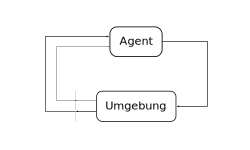
\includegraphics[height=0.5\textwidth, width=0.9\textwidth]{abbildungen/schnittstelle_agent_umgebung.pdf}
  \caption{Die Abbildung zeigt das Labyrinth der Umgebung \glqq Four\_Ways\_Many\_Goals\grqq{}. Der Agent startet zu Beginn jeder Episode auf dem zentralen Feld (rotes Dreieck) und erhält als Beobachtung einen Ausschnitt dem roten Rechteck entsprechend. Die grünen Kreise mit dem Buchstaben Z symbolisieren die möglichen Positionen zur Platzierung der Ziele.}
  \label{fig_fwmg_ep_start}
\end{figure}

Die Umgebung \glqq Four\_Ways\_Many\_Goals\_2D \grqq{} ist eine 2D-Umgebung im Stile eines Labyrinths. Sie verfügt über eine fixe Größe von 9 Feldern in horizontaler Richtung und 9 Feldern in vertikaler Richtung. Vom zentralen Punkt der Umgebung geht in jede der vier Richtungen ein Weg aus. Dieser Weg verzweigt sich dann ggf. noch ein weiteres mal. Auf jedem Weg gibt es eine Position zur Platzierung eines Ziels. Zu Beginn einer Episode werden auf diesen vier Position zwischen zwei und vier Ziele zufällig positioniert.

Diese Ziele verfügen wieder über eine eindeutige Nummer. Der Agent beginnt jede Episode auf dem zentralen Feld in der Mitte und startet für jede Episode neu bestimmten zufälligen Blickrichtung. Die Aufgabe des Agenten besteht wieder darin, die Ziele in der korrekten Reihenfolge abzulaufen. Die dafür verwendete Struktur der Rewards entsprecht der aus der vorherigen Umgebung. Lediglich die maximale Schrittanzahl unterscheidet sich. Für zwei Ziele stehen dem Agenten maximal XXX Schritte zur Verfügung, für drei Ziele YYY Schritte und für vier Ziele ZZZ Ziele.

Der Zustand $s_t$ ist hinsichtlich der binärkodierten Kanäle genau so aufgebaut wie bei der vorherigen Umgebung. Lediglich die Sichtreichweite in Blickrichtung wird um ein Feld reduziert, um der vermeintlich kleinen Umgebung genüge zu tragen. Somit ergibt sich die Größe des Zustands $s_t$ zu $(Anzahl_Ziele + 1) \times 3 \times 3$.

Bei dieser Umgebung wird der Agent im Vergleich zur vorherigen Umgebung zusätzlich mit Hindernissen konfrontiert.


\section{3D-Experiment}

Nachdem zuvor das Verhalten der Neural Map in verschiedenen 2D-Umgebungen ausführlich untersucht wurde, soll nun eine 3D-Umgebung verwendet werden.

Die 3D-Umgebung wird auf Basis von ViZDoom erstellt. ViZDoom basiert auf dem Computerspiel Doom und ermöglicht es, selbiges im RL Kontext zu benutzen.

Die Umgebung ist eine Adaption der 2D-Umgebung \glqq One\_Room\_Many\_Goals\grqq{}. Sie besteht somit aus einem quadratischem Raum. In diesem Raum werden zufällig zwei Ziele platziert, eine grüne Säule und eine rote Säule. Für die Platzierung der Ziele stehen insgesamt XXX mögliche Positionen zur Verfügung, wobei diese auf die beiden Raumhälften aufgeteilt sind. Zunächst wird zufällig eine dieser Positionen für das grüne Ziel ausgewählt. Um zu verhindern, dass die beiden Ziele zu nah beieinander liegen, stehen für die anschließende Platzierung des roten Ziels nur die Positionen in der anderen Raumhälfte zur Verfügung. Der Agent startet immer auf einer fixen Position in der Mitte des Raumes, die initiale Blickrichtung ist ebenfalls immer dieselbe. Die Aufgabe des Agenten ist es, zuerst zum grünen Säule und dann zur roten Säule zu laufen. Hierfür erhält er für das Erreichen der grünen Säule einen Reward von 0,2 und für das Erreichen der roten Säule einen Reward von 1,0. Dafür stehen dem Agenten XXX Schritte zur Verfügung. Für jeden Schritt erhält er wieder einen Living-Reward von $-1/Maximale\_Schrittanzahl.

Der Agent kann zwischen den drei Aktionen \glqq Drehung links\grqq{}, \glqqDrehung rechts\grqq{} und \glqq Gehe geradeaus\grqq{} auswählen. Dazu erhält er als Observation ein RGB-Array der Dimensionalität $120 \times 160 \times 3$.



\section{Untersuchung der Neural Map als reine Speicherstruktur}

Im folgenden Experiment soll die Neural Map außerhalb des bisherigen RL Kontexts untersucht werden. Es soll herausgefunden werden, inwiefern sich die Neural Map als reine Speicherstruktur nutzen lässt. Hierbei ist insbesondere von Interesse, inwiefern die Neural Map in ihrem internen Speicher eine Karte der Umgebung generieren kann. Um dies zu ergründen, wird eine leicht abgeänderte Form der Neural Map im Supervised Lernkontext betrachtet. Dazu werden folgende Annahmen getätigt. Zunächst wird wie in den 2D-Experimenten die vertikale und horizontale Größe des internen Speichers entsprechend der Umgebungsgröße gewählt. Somit entspricht eine Position in der Umgebung exakt einer Speicherposition. Die Informationen über die Umgebung, d.h. das Vorhandensein von Wänden bzw. freien Feldern und die Lage der Ziele, sind wie in den Abschnitten XXX und YYY beschrieben binär kodiert. Daraus ergibt sich, dass für jede Position der Umgebung ein entsprechend binärkodierter Umgebungsvektor existiert. Da es zu jeder Position in der Umgebung genau eine Position im internen Speicher gibt und sich das Feature an dieser Speicherposition nur durch seine Dimensionalität von dem Umgebungsvektor unterscheidet, wird das Feature als kodierte Form des Umgebungsvektors angesehen. Dabei ist die Kodierung zunächst unbekannt. Auf Basis dieser Annahmen wird für das Experiment eine leicht modifizierte Variante der Neural Map erstellt. Diese erhält als Eingabe wie gehabt eine Observation $s_t$ und den aktuellen Inhalt des internen Speichers $M_t$ und schätzt auf Basis dieser den Umgebungsvektor an der entsprechenden Position $(x_t, y_t)$. Im Fall der Neural Map mit der Erweiterung des Schreibvektors wird zusätzlich auch noch der Umgebungsvektor an der Position $(x_{ext_t},y_{ext_t})$ geschätzt. Im Folgenden wird wegen der besseren Lesbarkeit darauf verzichtet, immer darauf hinzuweisen, dass in Abhängigkeit der Benutzung des erweiterten Schreiboperators wahlweise ein oder zwei Vektoren von der modifizierten Variante der Neural Map geschätzt bzw. erzeugt werden.

Die für die Experimente benötigten Daten bilden Paare der Form (Eingabe, wahre Ausgabe). Um diese zu generieren, wird den 2D-Umgebungen eine zusätzliche Methode hinzugefügt. Diese erzeugt eine zufällige Observation aus der entsprechenden Umgebung. Dazu wird zunächst zufällig eine gültige Position des Agenten bestimmt, d.h. eine Position auf einem freien Feld. Anschließend wird auch die Orientierung zufällig gewählt und die zu der Positon und Orientierung gehörige Observation zurückgegeben. Da im Supervised Kontext auch die wahre Ausgabe bekannt sein muss, wird eine weitere Methode benötigt. Diese gibt die gesamte Umgebung zurück, d.h. die Umgebungsvektoren für alle Positionen, und wird einmal zu Beginn des Experiments aufgerufen. Im weiteren Verlauf können dann hieraus die jeweils benötigten Umgebungsvektoren auf Basis der Positionen extrahiert werden. Auf diese Weise werden die benötigten paarweisen Datenpunkte generiert.

Da die Neural Map nun als Ausgabe auch einen Vektor mit der gleichen Dimensionalität wie der Umgebungsvektor erzeugen muss, wird sie entsprechend modifiziert. Dazu wird zunächst das finale Neuronale Netz der Neural Map entfernt, da dessen Zweck in der Schätzung der Policy liegt und diese in diesem Experiment nicht benötigt wird. Das so veränderte Modell erzeugt als Ausgabe den Schreibvektor $w_{t+1}^{(x_t,y_t)}$ mittels der Local Write Operation. Da dieser noch über eine andere Dimensionalität als der Umgebungsvektor verfügt, wird er anschließend von einer weiteren Fully-Connected Schicht verarbeitet. Diese kann als Dekoder angesehen werden, da sie zur Schätzung des Umgebungsvektors das entsprechend kodierte Feature dekodiert. Somit generiert die entsprechend abgeänderte Neural Map als Ausgabe einen Vektor in der gleichen Dimensionalität wie der Umgebungsvektor. Damit die Einträge des geschätzten Umgebungsvektors auch aus dem Intervall $[0, 1]$ kommen, wird als Aktivierungsfunktion in der Dekoder-Schicht die Sigmoid-Funktion verwendet.

Nun kann wie im Supervised Kontext üblich die Ausgabe des Modells, also die Schätzung, mit der wahren Ausgabe verglichen werden, indem die Differenz der beiden Vektoren gebildet wird. Auf diesen Differenzvektor wird dann der mittlere quadratische Fehler angewendet. Die so entstehende Verlustfunktion kann nun mit einem entsprechenden Optimierer minimiert werden. Dazu berechnet selbiger den Gradienten des Modells und ändert auf Basis dessen die Parameter des Modells. Hierzu wird der sogenannte Adam Optimierer verwendet. Seine Parameter entsprechen den Standardwerten und als Lernrate wird $3e-4$ verwendet. Die Modelle werden jeweils für $25.000$ Schritte trainiert.

Für die Experimente wird zum einen die Umgebung \glqq One\_Room\_Many\_Goals\grqq{} in der Größe $9 \times 9$ mit 4 Zielen verwendet und die Umgebung \glqq Four\_Ways\_Many\_Goals\grqq{} ebenfalls mit 4 Zielen. Als Modelle werden die Grundvariante der Neural Map und die Variante mit der Erweiterung des Schreiboperators betrachtet. Von jeder der beiden Umgebungen werden 10 zufällige Konfigurationen verwendet, auf Basis derer die beiden Modelle trainiert werden. Eine Konfiguration entspricht dabei einer bestimmten Platzierung der 4 Ziele und wird paarweise für beide Modelle verwendet, um die entsprechenden Ergebnisse vergleichen zu können. Lediglich die zum Training verwendeten zufälligen Observationen unterscheiden sich noch. Nach dem Ende des Traingsprozesses wird abschließend die Güte der erzeugten Karte bewertet, indem für alle gültigen Position bzw. freien Felder die Differenz zwischen den geschätzten und tatsächlichen Umgebungsvektoren bestimmt wird und auf diesen anschließend der Mean-Squared-Error berechnet wird.

Die Abbildungen \ref{fig_mem_test_ormg} und \ref{fig_mem_test_fwmg} zeigen beispielhafte Verläufe des Mean-Squared-Errors über die Anzahl der Trainingschritte für die jeweiligen Umgebungen. Dabei ist auffällig, dass der MSE zu Beginn des Trainings relativ schnell bis ungefähr $0,2$ abfällt, ehe er dann für eine längere Zeit auf diesem Wert verweilt, bevor er wiederum weiter abfällt und seinen Endwert erreicht. In allen betrachteten Konfigurationen liegt der MSE am Ende des Trainings in der Größenordnung zwischen $10^-4$ und $10^-5$. Diese Werte werden auch bei der zuvor beschriebenen abschließenden Güteberechnung der Karte erreicht. Auch bei einer Sichtung der erzeugten Karten durch das menschliche Auge konnten die Positionen der Ziele fehlerfrei identifiziert werden, d.h. die entsprechende Eins in dem Umgebungsvektor war hinreichend signifikant.


\begin{figure}[ht!]
  \centering
  %\includegraphics[keepaspectratio,width=1.0\textwidth]{abbildungen/mem_test_ormg.pdf}
  \includegraphics[height=0.575\textwidth, width=0.9\textwidth]{abbildungen/mem_test_ormg.pdf}
  \caption{Die Abbildung zeigt die Entwicklung des Mean-Squared-Error über die Anzahl der Trainingschritte für die Neural Map und die Neural Map mit der Erweiterung des Schreiboperators für die Umgebung \glqq One\_Room\_Many\_Goals\grqq{}.}
  \label{fig_mem_test_ormg}
\end{figure}

\begin{figure}[ht!]
  \centering
  %\includegraphics[keepaspectratio,width=1.0\textwidth]{abbildungen/mem_test_fwmg.pdf}
  \includegraphics[height=0.575\textwidth, width=0.9\textwidth]{abbildungen/mem_test_fwmg.pdf}
  \caption{Die Abbildung zeigt die Entwicklung des Mean-Squared-Error über die Anzahl der Trainingschritte für die Neural Map und die Neural Map mit der Erweiterung des Schreiboperators für die Umgebung \glqq Four\_Ways\_Many\_Goals\grqq{}.}
  \label{fig_mem_test_fwmg}
\end{figure}
